\documentclass[a4paper]{article}

\usepackage[margin=1.1in]{geometry}
\usepackage[utf8]{inputenc}
%\usepackage[T1]{fontenc}
%\usepackage{textcomp}
\usepackage[spanish]{babel}
\usepackage{amsmath, amssymb}
\usepackage{amsthm}
\usepackage{braket}
\usepackage{graphicx}
\decimalpoint

\DeclareMathOperator{\R}{\mathbb{R}}
\DeclareMathOperator{\C}{\mathbb{C}}
\DeclareMathOperator{\N}{\mathbb{N}}
\DeclareMathOperator{\Z}{\mathbb{Z}}
\DeclareMathOperator{\Tr}{Tr}
\DeclareMathOperator{\tr}{tr}

\newtheorem{theorem}{Theorem}

\title{Delta function for $GF(p^{n})$}
\author{Ernesto Camacho Ramírez}
\begin{document}
  \maketitle

  We use the following definition of an eigenstate of an
  abelian curve $\Gamma = \{(\alpha(\tau),\beta(\tau)) :
  \tau \in F\}$ using the displacement operators:
  \begin{equation}
    \ket{\psi_\kappa^{\alpha,\beta}}
    \bra{\psi_\kappa^{\alpha,\beta}}
    = \frac{1}{p^{n}}
    \sum_{\tau}^{} \chi(\kappa\tau)
    D(\alpha(\tau),\beta(\tau)).
  \end{equation}
  By fixing a phase space and using the definition of the
  kernel in terms of the displacement operators:
  \begin{equation}
    w(\alpha,\beta)
    = \frac{1}{p^{n}} \sum_{\gamma,\delta}^{}
    \chi(\gamma\beta - \delta\alpha) D(\gamma,\delta),
  \end{equation}
  we can calculate the Wigner function for any eigenstate of
  commuting displacement operators.  Running through the
  calculations and using the fact the displacement operators
  have the correct phases (for odd characteristic the phases
  are unique) we obtain the following simplified expression
  for the Wigner function at the arbitrary point $(a,b)$:
  \begin{equation}
    \braket{
      \psi_{\kappa}^{\alpha,\beta}|w(a,b)|
      \psi_{\kappa}^{\alpha,\beta}
    }
    = \frac{1}{2^{n}}
    \sum_{\tau}^{}
    \chi\left( \alpha(\tau)b - \beta(\tau)a \right)
    \chi(\kappa\tau)
    = \sum_{\tau}^{} \delta_{a,\alpha(\tau)}
    \delta_{b,\beta(\tau)}.
  \end{equation}

  Consider the abelian curves of the $(0,9,0)$ set:
  \begin{equation}
    \alpha = \beta + \sigma^6 \beta^2 + \sigma^3 \beta^{4},
    \quad
    \beta = \alpha + \sigma^3 \alpha^2 + \sigma^5 \alpha^4.
  \end{equation}
  Their Wigner functions are shown in the following figures:

  \begin{figure}[ht]
    \centering
    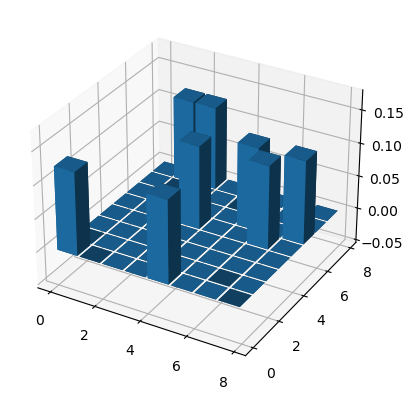
\includegraphics[width=0.5\textwidth]{090-1.png}
    \caption{$\alpha = \beta + \sigma^6 \beta^2 + \sigma^3 \beta^{4}$}
    \label{fig:090-1}
  \end{figure}

  \begin{figure}[ht]
    \centering
    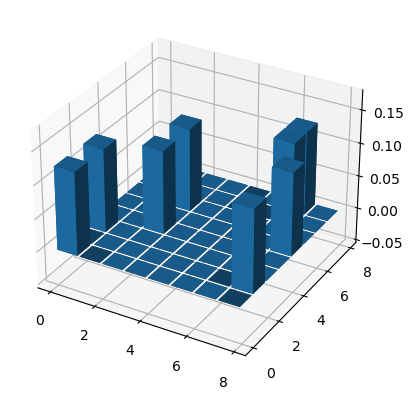
\includegraphics[width=0.5\textwidth]{090-2.png}
    \caption{$\beta = \alpha + \sigma^3 \alpha^2 + \sigma^5 \alpha^4$}
    \label{fig:090-2}
  \end{figure}

  As we can see the graphs represent delta functions
  corresponding to the curve. I expected that this would
  \textit{not} be the case for non-abelian curves, that is
  commutative curves for which the selected phases do
  \textit{not} satisfy the condition
  \begin{equation}
    D(\alpha(\tau),\beta(\tau))
    D(\alpha(\tau'),\beta(\tau'))
    = D(\alpha(\tau+\tau'),\beta(\tau+\tau')).
  \end{equation}
  But it seems that the abelian condition is not required
  in order for the Wigner function to be delta function!
  It seems that the only thing required is that the
  displacement operators have phases that match the selected
  phases of the rays. This can be seen by the example of the
  non-abelian curves from the same $(0,9,0)$ bundle:
  \begin{equation}
    \alpha = \sigma^6 \beta + \sigma^3 \beta^2 + \sigma^5
    \beta^{4},
    \quad
    \beta = \sigma^2 \alpha + \sigma^3 \alpha^2 + \sigma^5
    \alpha^{4}.
  \end{equation}
  Although these curves are not abelian, by simply assigning
  the phases given by the rays, we obtain delta functions:
  \begin{figure}[ht]
    \centering
    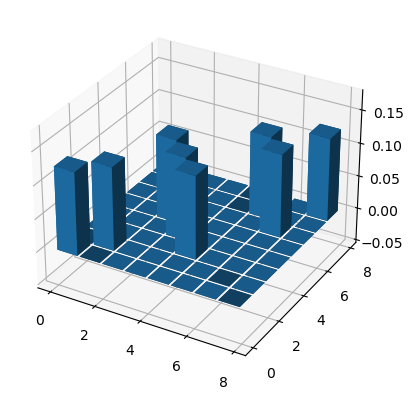
\includegraphics[width=0.5\textwidth]{090-3.png}
    \caption{$\alpha = \sigma^6 \beta + \sigma^3 \beta^2 + \sigma^5
    \beta^{4}$}
    \label{fig:090-3}
  \end{figure}
  \begin{figure}[ht]
    \centering
    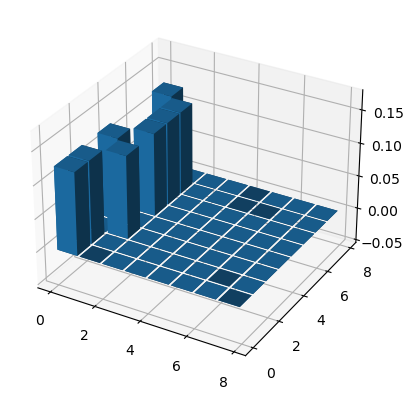
\includegraphics[width=0.5\textwidth]{090-4.png}
    \caption{$\beta = \sigma^2 \alpha + \sigma^3 \alpha^2 + \sigma^5
    \alpha^{4}$}
    \label{fig:090-4}
  \end{figure}

  The fact that the abelian condition is not satisfied means
  that the displacement operators indexed by the points of
  such a curve do not form a group. This does not affect the
  non-negativity of the eigenstates of such a set of
  commuting operators, but it must have other implications.
  Covariance maybe?

\end{document}
